\documentclass[sigconf,nonacm]{acmart}

\usepackage{fancyhdr}
\settopmatter{printacmref=false, printfolios=true}

\usepackage{graphicx}
\usepackage{booktabs}

\begin{document}

\title{The Edge Negotiator: Codes of Conduct for Decentralized Autonomous Traffic Optimization}

\author{25153651}
\affiliation{%
  \institution{University College London}
  \country{United Kingdom}
}

\begin{abstract}
This report proposes a Code of Conduct for the ``Edge Negotiator,'' a decentralized traffic optimization system where each intersection runs an autonomous Small Language Model on edge hardware. The system enables semantic reasoning about traffic priority, distinguishing an ambulance from routine congestion, while logging every decision to an immutable blockchain ledger for post-hoc audit. Five codes are proposed addressing algorithmic transparency, fail-safe override, data sovereignty, equitable service, and adversarial robustness. Two speculative scenarios, framed using Dunne and Raby's Future Cones~\cite{dunne2013}, explore consequences when codes are respected and broken, analysed through Meadows' leverage points~\cite{meadows1999}. The codes address a governance gap: the EU AI Act classifies road traffic AI as high-risk~\cite{euaiact}, yet no deployed system audits why a light turned green.
\end{abstract}

\keywords{decentralized traffic optimization, edge AI, blockchain auditability, small language models, IoT codes of conduct, speculative design}

\maketitle

\section{Part 1: The Edge Negotiator System}

\subsection{Use Case Scenario}

The \textbf{Edge Negotiator} replaces legacy centralized traffic control architectures such as SCATS and SCOOT, which govern over 60,000 intersections globally using 1980s heuristic logic~\cite{fairscosca}. SCOOT alone manages 4,500 of London's 6,400 signalised junctions~\cite{tfl2024}. These systems lack semantic understanding: they detect vehicle presence via induction loops but cannot reason about \textit{why} a vehicle should receive priority or weigh competing claims contextually.

The Edge Negotiator deploys a 3B-parameter Small Language Model (SLM), INT4-quantized, at each intersection on GPU-accelerated edge hardware, enabling local semantic reasoning without cloud dependency. The system operates through a four-stage pipeline: \textbf{Perceive} (cameras detect vehicles via YOLOv8 at 30+ FPS~\cite{yolov8}), \textbf{Reason} (the SLM evaluates priority via Chain-of-Thought reasoning), \textbf{Act} (the light changes immediately), and \textbf{Audit} (a cryptographic proof is logged asynchronously to a blockchain ledger). This ``Optimistic Execution with Post-Hoc Audit'' architecture resolves the tension between real-time responsiveness and verifiable trust: the decision executes in milliseconds while the proof is anchored within seconds.

\begin{figure}[h]
  \centering
  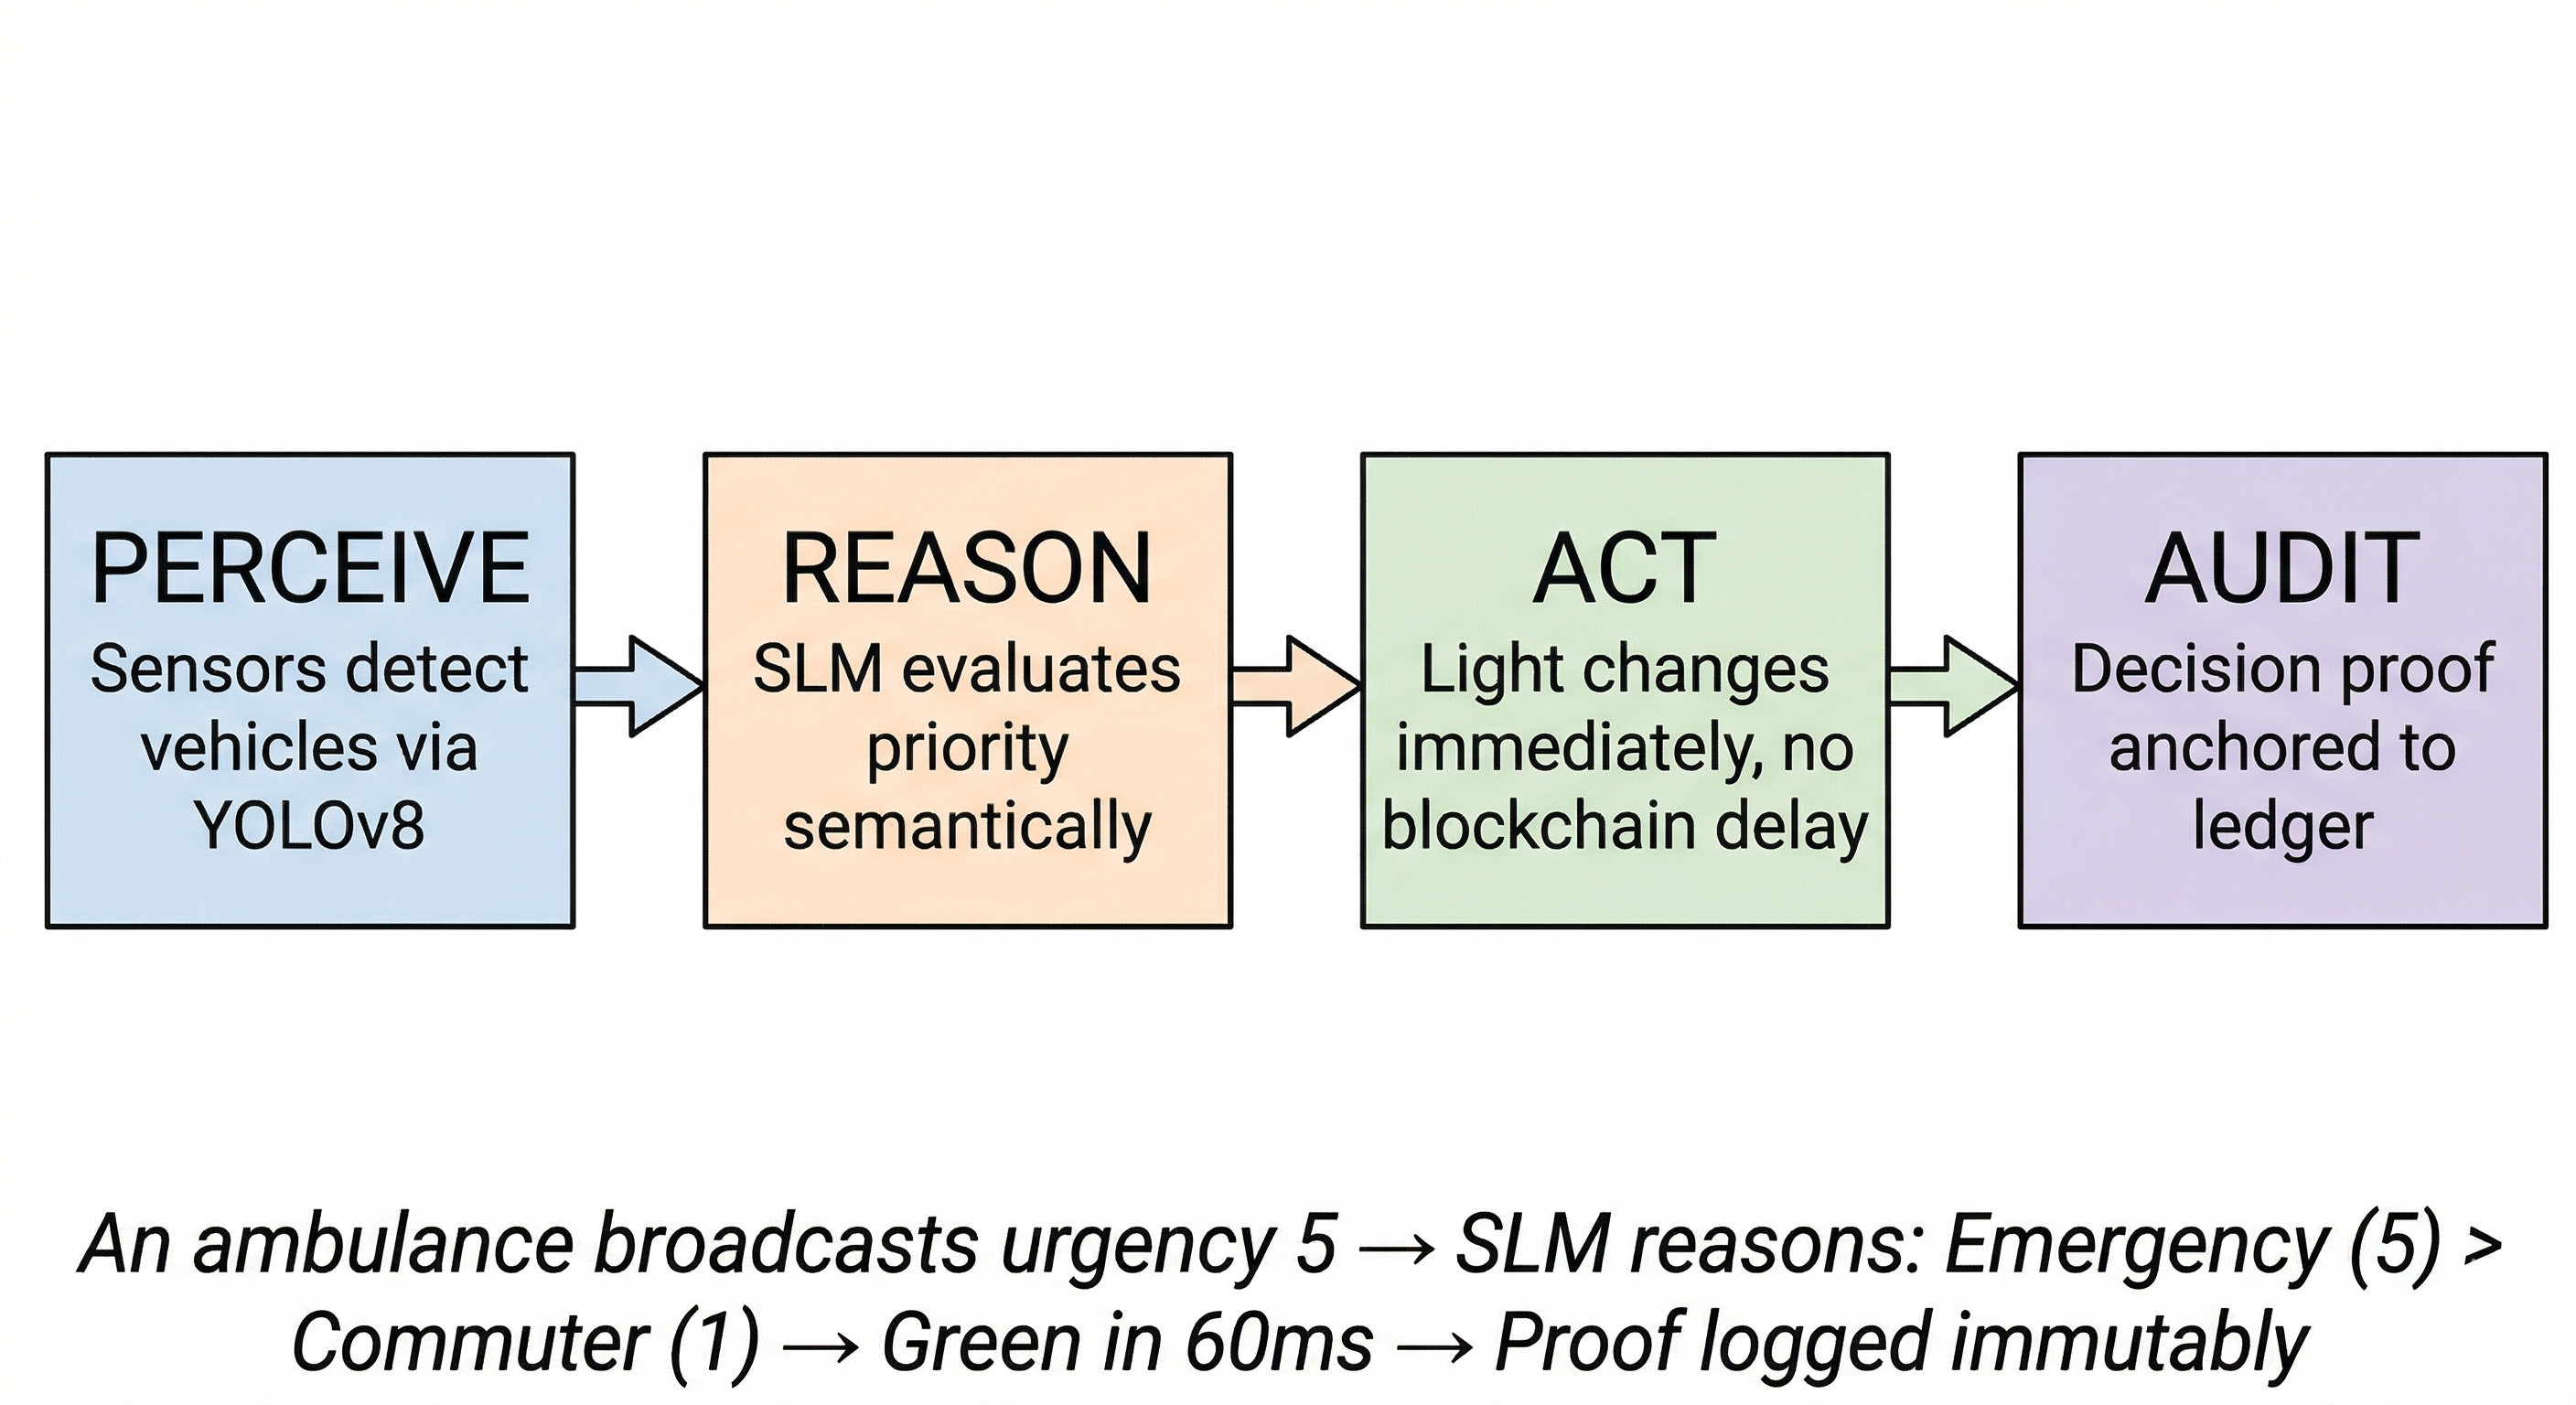
\includegraphics[width=\columnwidth]{fig1.png}
  \caption{The Edge Negotiator's four-stage pipeline. Decisions execute immediately; blockchain audit is asynchronous.}
  \label{fig:pipeline}
  \Description{A horizontal flowchart showing four connected boxes: Perceive, Reason, Act, and Audit, with an ambulance use case example below.}
\end{figure}

\textit{Example:} An ambulance broadcasts urgency~5. The SLM reasons: ``Emergency~(5) exceeds commuter traffic~(1).'' The light switches green in 60ms. The reasoning trace is signed and logged immutably for post-incident audit.

\subsection{Technical Features}

\textbf{Edge AI Inference.} Traffic-R1, a 3B foundation model for traffic signal control, is deployed in production managing signals for 55,000+ drivers daily while outperforming GPT-4o on zero-shot traffic benchmarks~\cite{trafficr1}. INT4-quantized SLMs achieve 20--40 tokens per second on the NVIDIA Jetson Orin Nano at 25W~\cite{nvidia2025}.

\textbf{Blockchain Audit Layer.} Rust-based Hyperledger Iroha~2 is designed for resource-constrained IoT environments~\cite{blockchain}. Java-based Hyperledger Besu, by contrast, requires a minimum of 8GB JVM heap and is architecturally infeasible on 8GB edge hardware~\cite{blockchain}. Decision proofs are cryptographically signed via ARM TrustZone~\cite{trustzone} and submitted for immutable storage.

\textbf{Deterministic Safety Layer.} A guardrail architecture between the SLM and signal actuator reduces execution of unsafe AI-generated plans from over 92\% to below 3\%~\cite{roboguard}.

\subsection{Context and Users}

The system targets urban intersections where autonomous vehicles, emergency services, public transit, cyclists, and pedestrians share road space. The ACM Code of Ethics mandates that systems becoming infrastructure carry heightened public-good responsibility (Principle~3.7)~\cite{acmcode}, and the EU AI Act Annex~III explicitly classifies AI in road traffic management as high-risk, mandating automatic decision logging from August 2026~\cite{euaiact}. Yet no deployed traffic system meets these requirements.

\section{Part 2: Codes of Conduct}

\begin{table}[h]
  \caption{Codes of Conduct for the Edge Negotiator system.}
  \label{tab:codes}
  \small
  \begin{tabular}{c p{1.8cm} p{4.2cm}}
    \toprule
    N & Title & Summary \\
    \midrule
    1 & Algorithmic Transparency \& Accountability & Every AI decision must produce a human-readable reasoning trace, signed and stored immutably on the blockchain ledger. \\
    2 & Fail-Safe Manual Override & A deterministic safety layer overrides the AI if commands violate physical safety constraints. Humans can always intervene. \\
    3 & Data Sovereignty \& Edge-First Processing & All sensor data is processed locally on edge hardware. Only hashed decision proofs leave the device, never raw data. \\
    4 & Equitable Service Provision & Priority is based on urgency and safety, not geography or wealth. The algorithm must not systematically disadvantage any group. \\
    5 & Adversarial Robustness & The system must resist spoofed signals, adversarial vision attacks, and attempts to game the negotiation protocol. \\
    \bottomrule
  \end{tabular}
\end{table}

\subsection{Code 1: Algorithmic Transparency \& Accountability}

Every traffic decision must produce a Chain-of-Thought reasoning trace linking observed state to action taken. This addresses the ``responsibility gap''~\cite{matthias2004}, and specifically the ``public accountability gap'' where citizens cannot obtain explanations for algorithmic decisions affecting public services~\cite{santoni2021}. The Edge Negotiator resolves this by generating semantic justifications such as \textit{``Ambulance on Lane~2 blocked; extending Green Phase~3,''} cryptographically signed and anchored to the blockchain as an ``ethical black box''~\cite{winfield2017}. The EU AI Act Article~12 mandates event logging for high-risk AI~\cite{euaiact}, and the Netherlands' national algorithm register, with 1,300+ algorithms from 500+ organisations~\cite{algorithmregister}, demonstrates that transparency at scale is operationally feasible.

\subsection{Code 2: Fail-Safe Manual Override}

The SLM is treated architecturally as an \textit{untrusted} performance optimiser following the Simplex pattern, where deterministic safety functions operate alongside the AI~\cite{nesti2025}. If the SLM commands ``Green'' but sensors detect vehicles clearing the intersection, the safety layer triggers an all-red emergency phase. This is necessary because LLMs can generate plausible control rationales that conflict with physical constraints and sensor data~\cite{mowbray2026}, and IEC~61508-3 does not recommend AI above SIL~1~\cite{iec61508}. Traffic engineers also retain physical override via a hardware kill switch. The real-world urgency is clear: in the ``Green Lights Forever'' attack, researchers compromised nearly 100 intersections from a single laptop via unencrypted wireless and factory-default credentials~\cite{ghena2014}. Failsafes against both AI failure and external compromise are essential, aligning with the BCS duty of ``due regard for public health, privacy, security and wellbeing''~\cite{bcs}.

\subsection{Code 3: Data Sovereignty \& Edge-First Processing}

All sensor data is processed locally on edge hardware. The perception pipeline converts camera frames into anonymised structured descriptions such as \textit{``15 cars northbound, 1 bus, 0 pedestrians,''} and only hashed decision proofs leave the device. This responds to documented surveillance overreach: San Diego's 3,300 smart streetlights, deployed for traffic analysis at \$30.23 million, were repurposed for law enforcement without public consent, ultimately provoking the TRUST SD Coalition campaign that forced the city to suspend data collection~\cite{sandiego}. The EDPB establishes that GDPR applies to all video cameras processing personal data, and generic purposes like ``safety'' are insufficient under Article~5(1)(b)~\cite{edpb2020}. Edge-first processing ensures identifiable imagery never enters a network.

\subsection{Code 4: Equitable Service Provision}

The algorithm must assign priority based on urgency and safety, never geography or wealth. Current signal timing embeds structural bias: standard software does not compute pedestrian delay, producing average vehicle waits of 20 seconds versus 80 seconds for pedestrians~\cite{nchrp969}. This vehicular bias maps onto inequality. In the US, per-capita pedestrian fatality rates in the lowest-income census tracts are over four times higher than in areas with median income above \$100,000~\cite{dangerousbydesign}. In London, people from the most deprived postcodes face nearly double the risk of being killed or seriously injured on the roads~\cite{tflequity}. Standard reinforcement learning for traffic inherently neglects fairness when maximising aggregate throughput~\cite{raeis2021}. The blockchain's immutable log enables equity audits, verifying equivalent service across neighbourhoods rather than optimising aggregate metrics.

\subsection{Code 5: Adversarial Robustness}

The system must defend against attacks on perception and reasoning pipelines. Adversarial stickers achieve 100\% misclassification of stop signs in laboratory settings and 84.8\% in field tests~\cite{eykholt2018}. Ben-Gurion University's ``phantom attacks'' used a \$300 projector on a digital billboard to display a phantom stop sign for 125 to 500 milliseconds, causing Tesla Autopilot to brake while leaving no physical evidence~\cite{nassi2020}. Adversarial patches achieve 76\% attack success against vision-language models, with pedestrian detection dropping 71.1 percentage points~\cite{fernandez2025}. The Edge Negotiator mitigates these through architectural separation: YOLOv8 detects object \textit{classes} without reading text, while the SLM reasons only over structured text descriptions, neutralising visual prompt injection. Secure Boot via the TEE prevents model poisoning.

\begin{figure}[h]
  \centering
  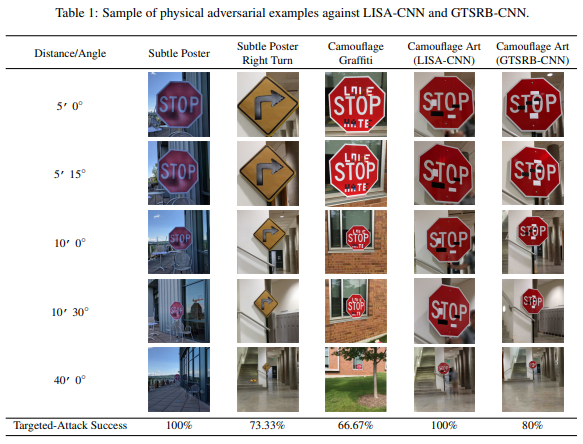
\includegraphics[width=\columnwidth]{fig2.png}
  \caption{Physical adversarial examples against traffic sign classifiers at varying distances. Reproduced from Eykholt et al.~\cite{eykholt2018}.}
  \label{fig:adversarial}
  \Description{A table of photos showing stop signs with adversarial stickers at different distances and angles, with attack success rates at the bottom.}
\end{figure}

\section{Part 3: Future Scenarios}

\begin{figure}[h]
  \centering
  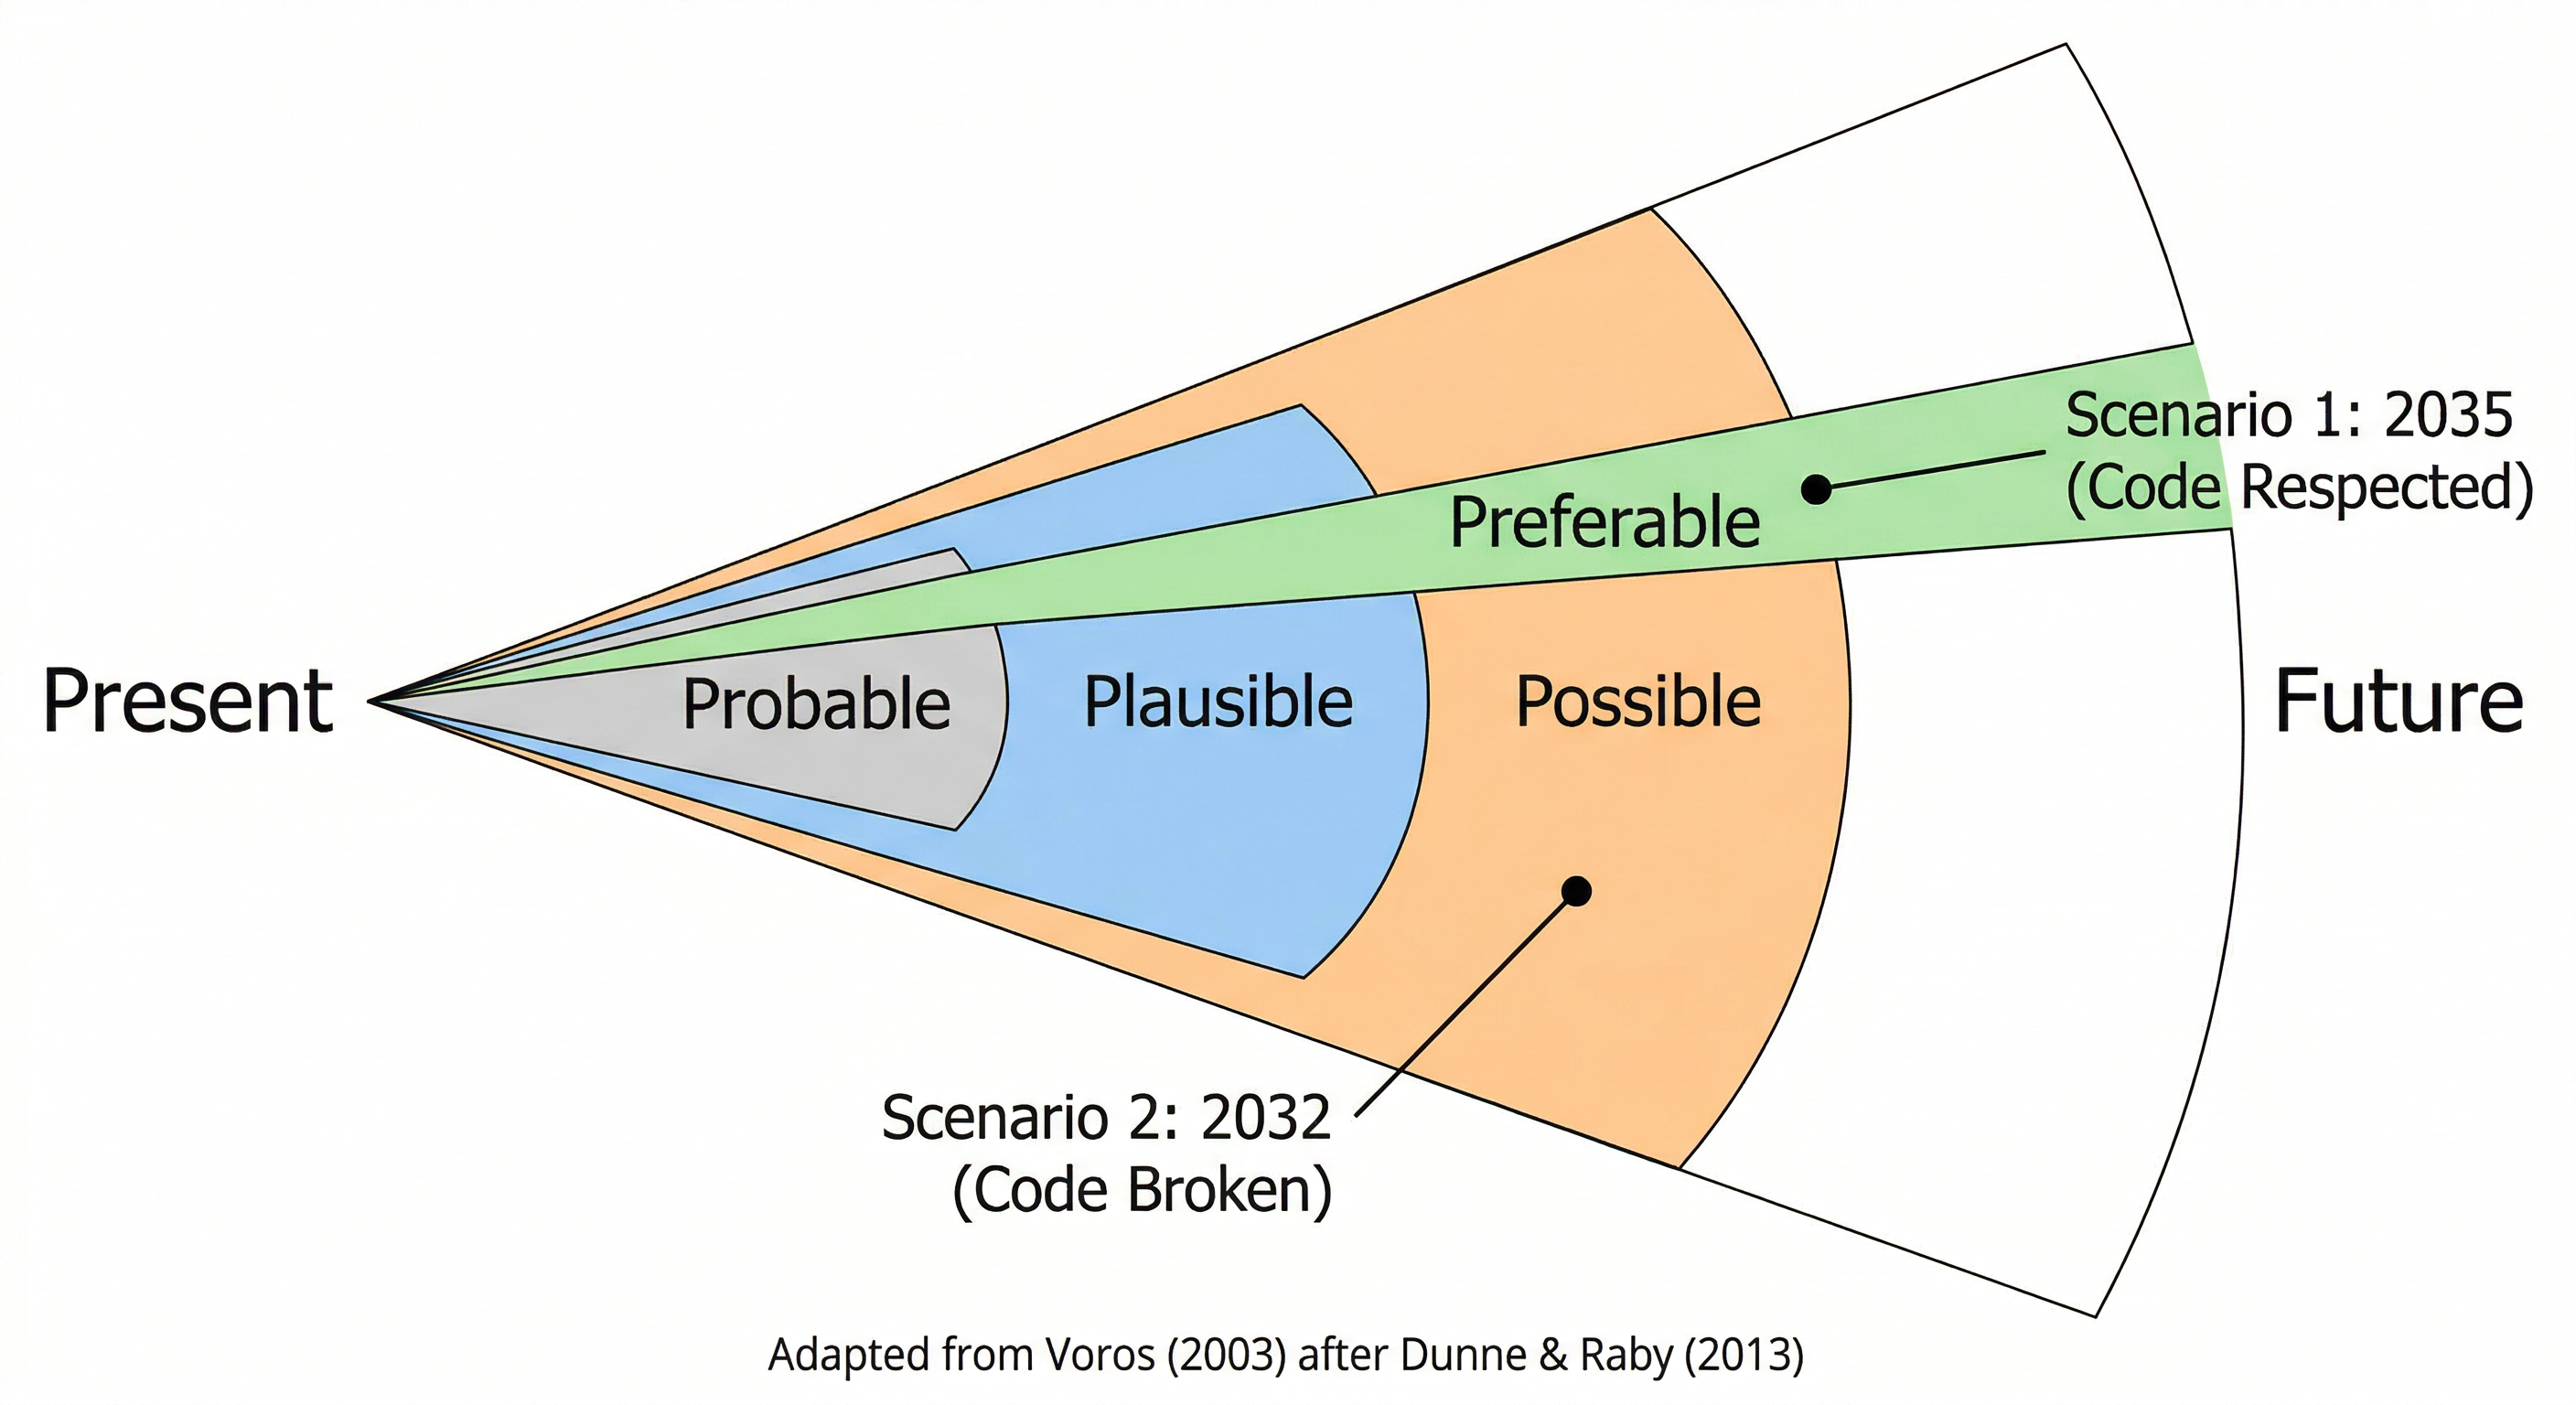
\includegraphics[width=\columnwidth]{fig3.png}
  \caption{Future Cones framework with both scenarios plotted. Adapted from Voros (2003) after Dunne \& Raby~\cite{dunne2013}.}
  \label{fig:cones}
  \Description{A futures cone diagram showing nested cones for probable, plausible, possible, and preferable futures, with Scenario 1 (2035) in the preferable band and Scenario 2 (2032) in the possible cone.}
\end{figure}

\subsection{Scenario 1: Code Respected --- Algorithmic Transparency (Preferable Future, 2035)}

London, 2035. The city's 6,400 signalised intersections, formerly managed by opaque SCOOT controllers, now run Edge Negotiator nodes. After a collision at Euston Road, Transport for London queries the blockchain and retrieves the full decision chain: Junction~14's SLM identified a delivery van running a red light and triggered evasive re-phasing, prioritising pedestrian safety (urgency~8) over traffic flow (urgency~2). The immutable log is presented in a public inquiry and the manufacturer's liability is established within days. Insurance companies offer reduced premiums for auditable AI routes. Compliance with EU AI Act Article~12 (effective since August 2026) has transformed regulatory burden into competitive advantage. Other cities procure nodes because every light change has a queryable justification: 1.2 billion decisions, each with a cryptographic audit trail.

\subsubsection{Context and Explanation}

This scenario occupies the \textbf{preferable} future cone~\cite{dunne2013}. It illustrates a reinforcing feedback loop: transparency enables trust, trust drives adoption, adoption generates data, and data improves the system. This operates at Meadows' leverage point~6 (information flows)~\cite{meadows1999}. The blockchain's role as an ``ethical black box''~\cite{winfield2017} resolves the liability deadlock currently stalling autonomous infrastructure deployment. The economic incentive (insurance premium reduction) demonstrates that governance codes generate commercial value, not merely compliance cost. The scenario is grounded in real precedent: in 2026, the University of Southampton and Minima Blockchain demonstrated the world's first blockchain-based ``black box'' on autonomous drone hardware during live flight~\cite{southampton2026}.

\subsection{Scenario 2: Code Broken --- Adversarial Robustness (Possible Future, 2032)}

Manchester, 2032. Criminals discover that adversarial patterns displayed on digital billboards fool the vision pipeline into hallucinating ``ghost vehicles.'' The system grants green corridors to empty lanes while genuine traffic is held at red. Organised theft rings exploit the manufactured gridlock to isolate delivery vehicles. The exploit spreads on social media and copycats in Birmingham and Leeds replicate it within days. The city disables the AI entirely, reverting to 1990s fixed-timing plans. Commuters lose 45 minutes daily. A parliamentary inquiry concludes the failure was architectural: the vendor shipped a monolithic vision-reasoning pipeline in which adversarial visual inputs directly influenced semantic reasoning, rather than the separated architecture Code~5 prescribes. The parallel to Ghena and Halderman's 2014 compromise of nearly 100 intersections from a single laptop~\cite{ghena2014} is inescapable: the attack surface was known and the defence was omitted.

\subsubsection{Context and Explanation}

This scenario occupies the \textbf{possible} future cone~\cite{dunne2013}: it requires no new physics but depicts an outcome contingent on specific failure modes. It illustrates how cascading trust collapse unfolds: a single exploit at one node propagates system-wide failure, a dynamic characteristic of tightly coupled decentralized systems~\cite{witthaut2022}. The attack vector is grounded in real research: physical adversarial attacks achieve 100\% success against some commercial vehicles~\cite{wang2025}, and phantom attacks leave no trace~\cite{nassi2020}. Code~5's architectural separation operates at Meadows' leverage point~5 (rules of the system)~\cite{meadows1999}. Changing the pipeline architecture is a higher-leverage intervention than adjusting any parameter within a monolithic design.

\section*{Concluding Statement}

The five codes are not confined to traffic optimisation. Any IoT system making autonomous decisions affecting public safety, whether smart grids distributing power, autonomous drones navigating airspace, or hospital monitoring systems triaging alerts, faces the same ``responsibility gap''~\cite{matthias2004} where accountability collapses without an identifiable decision-maker. Three structural problems converge. Professional codes (BCS, ACM) presuppose bilateral accountability relationships that dissolve in decentralized meshes. Transparency requirements exist (EU AI Act Article~12, IEEE~7001~\cite{winfield2022ieee}) but no deployed traffic system meets them. And the attack surface, from adversarial stickers to factory-default credentials, exceeds what ``follow accepted best practices'' can address.

The speculative scenarios reveal an asymmetry: trust is slow to build and fast to destroy. Transparency (Code~1) creates reinforcing feedback loops at leverage point~6; adversarial failure (Code~5) triggers cascading collapse. These dynamics characterise complex systems near criticality~\cite{witthaut2022}.

The ``act first, prove later'' blockchain audit pattern offers transferable architecture, but the codes encode normative choices. Signal timing software that does not compute pedestrian delay~\cite{nchrp969} already embeds a value judgment about whose time matters. A Code of Conduct optimising for vehicle throughput produces a fundamentally different city than one optimising for equitable accessibility~\cite{martens2016}. The most important design decision is not which algorithm to deploy, but which values to encode in its governance.

\begin{thebibliography}{35}

\bibitem{dunne2013}
A. Dunne and F. Raby, \textit{Speculative Everything: Design, Fiction, and Social Dreaming}. MIT Press, 2013.

\bibitem{meadows1999}
D. Meadows, ``Leverage Points: Places to Intervene in a System,'' \textit{Sustainability Institute}, 1999.

\bibitem{euaiact}
Regulation (EU) 2024/1689 of 13 June 2024, Laying Down Harmonised Rules on Artificial Intelligence (EU AI Act). Annex~III, Section~2: road traffic management classified as high-risk. Article~12: automatic event logging. Effective 2 August 2026.

\bibitem{fairscosca}
FairSCOSCA, ``Fairness At Arterial Signals --- Just Around The Corner,'' arXiv:2601.06275, 2026.

\bibitem{tfl2024}
Transport for London, ``Traffic signals and crossings,'' tfl.gov.uk, 2024.

\bibitem{yolov8}
G. Jocher, A. Chaurasia, and J. Qiu, ``Ultralytics YOLO,'' 2023.

\bibitem{trafficr1}
Z. Zou et al., ``Traffic-R1: A 3B Foundation Model for Traffic Signal Control via Agentic Reinforcement Learning,'' arXiv:2508.02344, August 2025.

\bibitem{nvidia2025}
NVIDIA Corporation, ``Jetson Orin Nano Super Developer Kit: AI Performance Benchmarks,'' NVIDIA Developer Documentation, January 2025.

\bibitem{blockchain}
D. Loghin et al., ``Blockchain Goes Green? Part~II: Characterizing the Performance and Cost of Blockchains on the Cloud and at the Edge,'' \textit{ACM Distributed Ledger Technologies}, 2024; Hyperledger Foundation, ``Besu System Requirements,'' besu.hyperledger.org, 2024.

\bibitem{trustzone}
S. Pinto and N. Santos, ``Demystifying Arm TrustZone: A Comprehensive Survey,'' \textit{ACM Computing Surveys}, vol.~51, no.~6, article~130, 2019.

\bibitem{roboguard}
Z. Ravichandran, A. Robey, V. Kumar, G.~J. Pappas, and H. Hassani, ``RoboGuard: A Provably Safe Guardrail Architecture for LLM-Based Robotic Systems,'' \textit{IEEE Robotics and Automation Letters}, 2025.

\bibitem{acmcode}
D. Gotterbarn et al., ``ACM Code of Ethics and Professional Conduct,'' Association for Computing Machinery, 2018.

\bibitem{matthias2004}
A. Matthias, ``The Responsibility Gap: Ascribing Responsibility for the Actions of Learning Automata,'' \textit{Ethics and Information Technology}, vol.~6, pp.~175--183, 2004.

\bibitem{santoni2021}
F. Santoni de Sio and G. Mecacci, ``Four Responsibility Gaps with Artificial Intelligence,'' \textit{Philosophy \& Technology}, vol.~34, no.~4, pp.~1057--1084, 2021.

\bibitem{winfield2017}
A. Winfield and M. Jirotka, ``The case for an ethical black box,'' in \textit{Proc. TAROS}, Springer LNCS vol.~10454, pp.~262--273, 2017.

\bibitem{algorithmregister}
City of Amsterdam, ``Algorithm Register,'' 2020; City of Helsinki, ``AI Register,'' 2020; Netherlands national \textit{Algoritmeregister}, 2022.

\bibitem{nesti2025}
F. Nesti et al., ``The Use of the Simplex Architecture to Enhance Safety in Deep-Learning-Powered Autonomous Systems,'' arXiv:2509.21014, 2025.

\bibitem{mowbray2026}
M. Mowbray et al., ``Neuro-Symbolic Verification for Preventing LLM Hallucinations in Process Control,'' \textit{Processes}, vol.~14, no.~2, article~322, 2026.

\bibitem{iec61508}
IEC 61508-3:2010, ``Functional safety of E/E/PE safety-related systems --- Part~3: Software requirements.''

\bibitem{ghena2014}
B. Ghena, W. Beyer, A. Hillaker, J. Pevarnek, and J.~A. Halderman, ``Green Lights Forever: Analyzing the Security of Traffic Infrastructure,'' in \textit{Proc. USENIX WOOT}, 2014.

\bibitem{bcs}
BCS, The Chartered Institute for IT, ``BCS Code of Conduct,'' current edition, bcs.org.

\bibitem{sandiego}
City of San Diego, ``Smart Streetlight Program Review and Policy Update,'' Office of the City Auditor, 2020.

\bibitem{edpb2020}
European Data Protection Board, ``Guidelines 3/2019 on Processing of Personal Data through Video Devices,'' Version~2.0, January 2020.

\bibitem{nchrp969}
NCHRP Report~969, \textit{Traffic Signal Control Strategies for Pedestrians and Bicyclists}, Transportation Research Board, 2022.

\bibitem{dangerousbydesign}
Smart Growth America, ``Dangerous by Design 2024,'' 2024.

\bibitem{tflequity}
Transport for London, ``New data shows people living in London's most deprived areas are twice as likely to be killed or seriously injured in road collisions,'' TfL Press Release, April 2023; P. Edwards et al., ``Serious injuries in children: variation by area deprivation and settlement type,'' \textit{Archives of Disease in Childhood}, 2008.

\bibitem{raeis2021}
M. Raeis and A. Leon-Garcia, ``A Deep Reinforcement Learning Approach for Fair Traffic Signal Control,'' in \textit{Proc. IEEE ITSC}, pp.~2512--2518, 2021.

\bibitem{eykholt2018}
K. Eykholt et al., ``Robust Physical-World Attacks on Deep Learning Models,'' in \textit{Proc. IEEE CVPR}, pp.~1625--1634, 2018.

\bibitem{nassi2020}
B. Nassi et al., ``Phantom of the ADAS: Securing Advanced Driver-Assistance Systems from Split-Second Phantom Attacks,'' in \textit{Proc. ACM CCS}, pp.~293--308, 2020.

\bibitem{fernandez2025}
D. Fernandez et al., ``Comparative Analysis of Patch Attack on VLM-Based Autonomous Driving Architectures,'' arXiv:2603.08897, 2025.

\bibitem{southampton2026}
University of Southampton and Minima Blockchain, ``World's First Blockchain-Based Black Box for Autonomous Drones,'' press release, March 2026.

\bibitem{witthaut2022}
D. Witthaut et al., ``Collective nonlinear dynamics and self-organization in decentralized power grids,'' \textit{Reviews of Modern Physics}, vol.~94, no.~1, 015005, 2022.

\bibitem{wang2025}
J. Wang et al., ``Large-Scale Measurement of Adversarial Attacks Against Commercial Traffic Sign Recognition,'' in \textit{Proc. NDSS}, 2025.

\bibitem{winfield2022ieee}
A. Winfield et al., ``An Ethical Black Box for Social Robots: a draft Open Standard,'' arXiv:2205.06564, 2022; IEEE~7001-2021, ``IEEE Standard for Transparency of Autonomous Systems.''

\bibitem{martens2016}
K. Martens, \textit{Transport Justice: Designing Fair Transportation Systems}. Routledge, 2016.

\end{thebibliography}

\end{document}
